\documentclass[12pt,twoside]{article}
\usepackage{mathtools} % for DeclareParedDelimiter
\usepackage{listings}
\usepackage{graphicx} % Required for including images
\newcommand{\reporttitle}{Foundations of Machine Learning}
\newcommand{\reportauthor}{Lionel Ngoupeyou Tondji}
\newcommand{\reporttype}{Assignment: Statistics and Probability}
\newcommand\myeq{\mathrel{\overset{\makebox[0pt]{\mbox{\normalfont\tiny\sffamily iid}}}{=}}}





\begin{document}
% front page

% Last modification: 2016-09-29 (Marc Deisenroth)
\begin{titlepage}
\newcommand{\HRule}{\rule{\linewidth}{0.5mm}} % Defines a new command for the horizontal lines, change thickness here


%----------------------------------------------------------------------------------------
%	LOGO SECTION
%----------------------------------------------------------------------------------------

\begin{center}

\includegraphics[height = 2cm]{qla}\hspace{4mm}

\includegraphics[height=2cm]{aims-rwanda}
\end{center}
 

\begin{center} % Center remainder of the page

%----------------------------------------------------------------------------------------
%	HEADING SECTIONS
%----------------------------------------------------------------------------------------
\textsc{\LARGE \reporttype}\\[1.5cm] 
\textsc{\Large African Institute for Mathematical Sciences}\\[0.5cm] 
\textsc{\large Quantum Leap Africa}\\[0.5cm] 
%----------------------------------------------------------------------------------------
%	TITLE SECTION
%----------------------------------------------------------------------------------------

\HRule \\[0.4cm]
{ \huge \bfseries \reporttitle}\\ % Title of your document
\HRule \\[1.5cm]
\end{center}
%----------------------------------------------------------------------------------------
%	AUTHOR SECTION
%----------------------------------------------------------------------------------------

\begin{minipage}{0.4\hsize}
 \begin{flushleft} \large
 \textit{Author: Lionel Ngoupeyou Tondji}\\
 \end{flushleft}
  \vspace{2cm}
 \makeatletter
 Date: \@date 
\end{minipage}
\vfill % Fill the rest of the page with whitespace



\makeatother

\end{titlepage}




\section{Linear Regression}
\subsection*{a) }
\subsubsection*{1)}
Let us find the maximum likelihood solution for the parameters $\sigma^2$ and $w$ in terms of $\Phi$.\\
In this question we consider a factorizing likelihood :
\begin{equation*}
p(y|x) = \prod_{i=1}^{N} p(y_i|x_i)
\end{equation*}
and Gaussian linear model :
\begin{equation*}
y_i  \sim \mathcal{N}(w^T \phi(x_i), \sigma^2)
\end{equation*}

Our goal is to Find the parameters that maximize the likelihood $p(x| \theta)$.\\
The step of finding the maximum are :
\begin{itemize}
	\item  Compute gradient with respect to θ
	\item  Set gradient to 0
	\item  Solve for θ
\end{itemize}

So we have :
\begin{equation*}
p(y| x) = \prod_{i=1}^{N} p(y_i| x_i) = \prod_{i=1}^{N} \mathcal{N}(w^T \phi(x_i), \sigma^2)
\end{equation*}

But instead of maximizing the Likelihood, we will maximize the log-Likelihood because log is a strictly monotonically function increasing function.

Why are we allow to this transformation? because
\begin{itemize}
	\item  We will obtain The same maximum
	\item  Gradients easy
	\item  Fewer numerical problems
\end{itemize}

Thus, the Log Likelihood is given by :
\begin{align*}
log \,p(y| x) &= log \, \prod_{i=1}^{N} p(y_i| x) \\
&= \sum_{i=1}^{N} log \, \left( \frac{1}{\sqrt{2 \pi \sigma^2}} exp\big(-\frac{1}{2 \sigma^2}\big(y_i - w^T \phi(x_i)\big)^2\big) \right) \\
&= -\frac{N}{2} log\big(2 \pi \sigma^2\big) + \sum_{n=1}^{N}  \, \left( -\frac{1}{2 \sigma^2}\big(y_i - w^T \phi(x_i)\big)^2 \right) \\
\end{align*}

The gradient of the Log Likelihood with respect to $\alpha = \sigma^2$ is given by :
\begin{align*}
\frac{\partial}{\partial \alpha}log \,p(y| x) &= \frac{\partial}{\partial \alpha}  \left( -\frac{N}{2} log\big(2 \pi \alpha\big) + \sum_{n=1}^{N}  \, \left( -\frac{1}{2 \alpha}\big(y_i - w^T \phi(x_i)\big)^2 \right) \right) \\
&= -\frac{N}{2 \alpha} + \frac{1}{2 \alpha } \sum_{i=1}^{N} \left( y_i - w^T \phi(x_i)\right)   \\
\end{align*}

Setting the gradient that we compute before to zero, we obtain:
\begin{equation*}
-\frac{N}{2 \alpha} + \frac{1}{2 \alpha^2 } \sum_{i=1}^{N} \left( y_i - w^T \phi(x_i)\right) = 0 \\
\Longrightarrow  -N \alpha + \sum_{i=1}^{N} \left( y_i - w^T \phi(x_i)\right) = 0
\end{equation*}

So we obtain :
\begin{equation}
\boxed{ \sigma^2 _{ML} = \frac{1}{N} \sum_{i=1}^{N} \left( y_i - w^T \phi(x_i)\right) }
\end{equation}

The gradient of the Log Likelihood with respect to $w$ is given by :
\begin{align*}
\frac{\partial}{\partial w}log \,p(y| x) &= \frac{\partial}{\partial w}  \left( -\frac{N}{2} log\big(2 \pi \sigma^2\big) + \sum_{n=1}^{N}  \, \left( -\frac{1}{2 \sigma^2}\big(y_i - w^T \phi(x_i)\big)^2 \right) \right) \\
&= -\frac{1}{2 \sigma^2} \frac{\partial}{\partial w}  \left( \sum_{n=1}^{N}  \, \left( y_i - w^T \phi(x_i)\right)^2  \right)   \\
&= -\frac{1}{2 \sigma^2} \frac{\partial}{\partial w} \Arrowvert \underbrace{ y - \phi(x)w }_{e}\Arrowvert^2\\
&= -\frac{1}{2 \sigma^2} \frac{\partial}{\partial w} \underbrace{\Arrowvert e(w) \Arrowvert ^2}_{L(e)}\\
\end{align*}

By using the Chain-rule, with $L(e) = \Arrowvert e(w) \Arrowvert ^2$ and $e(w) = y - \phi(x)w$, we obtain : 
\begin{align*}
\frac{\partial}{\partial w}log \,p(y| x) &= -\frac{1}{2 \sigma^2} \frac{\partial}{\partial w}L(e)\\ \\
										 &= -\frac{1}{2 \sigma^2}\frac{\partial}{\partial e}L(e)\frac{\partial}{\partial w}e \\ \\
										 & = -\frac{1}{2 \sigma^2}  \left(2e^T\right) \left(-\phi(x)\right) \\ \\
										 &= \frac{1}{\sigma^2}  \left(y - \phi(x)w\right)^T \phi(x) \\ \\
\end{align*}

Setting the gradient that we compute before to zero, we obtain:
\begin{equation*}
\frac{1}{\sigma^2}  \left(y - \phi(x)w\right)^T \phi(x) = 0 \\
\Longrightarrow  y^T\phi(x) - w^T\phi(x)^T\phi(x) = 0
\end{equation*}

\begin{equation*}
\Longrightarrow   w^T\phi(x)^T\phi(x) = y^T\phi(x)
\end{equation*}

\begin{equation*}
\Longrightarrow   w^T = y^T\phi(x) \left(\phi(x)^T\phi(x)\right)^{-1} \\
\end{equation*}

\begin{equation*}
\Longrightarrow   w = \left(\phi(x)^T\phi(x)\right)^{-1}\phi(x)^Ty  \\
\end{equation*}

So we obtain :
\begin{equation}
\boxed{  w_{ML} = \left(\phi(x)^T\phi(x)\right)^{-1}\phi(x)^Ty  }
\end{equation}
\\
%\vspace{7cm}
\subsubsection*{2)} Let us have a look at on the data set
\begin{center}
	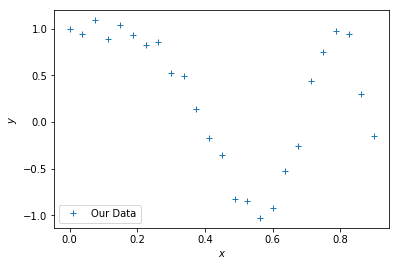
\includegraphics{../data}	     
\end{center}



Plot the predictive mean at test points in the interval $[−0.3, 1.3]$ in
the case of polynomial basis functions of order 0, 1, 2, 3 and also order 11. Plot all the curves on the same axes, showing also the data.

\begin{center}
	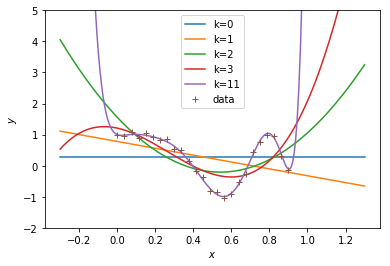
\includegraphics{../index}	     
\end{center}

\subsection*{b)} Repeat the previous part but this time with trigonometric basis functions of orders 1 and 11. Use test points in $[-1, 1.2]$ to see the periodicity. Note that your basis functions should be of size $2J + 1$ for order $J$ (i.e. don’t forget the bias term).

\begin{center}
	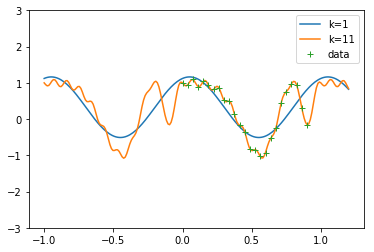
\includegraphics{../index1}	     
\end{center}

\subsection*{c)} In this part we will investigate over-fitting with leave-one-out cross validation. We should use trigonometric basis functions of order 0 to 10 inclusive and for each choice use leave-one-out cross validation to estimate the average squared test error. Plot this average error on a graph against order of basis together. On the same graph plot also the maximum likelihood value for $\sigma^2$.

\begin{center}
	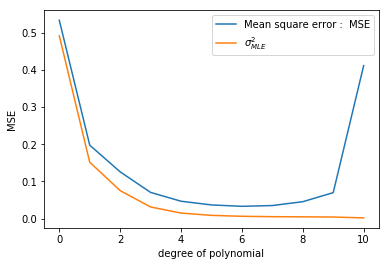
\includegraphics{../index2}	     
\end{center}

\section*{d)} Briefly describe the concept of over-fitting, using your graph in the previous part as an illustrative example. You should also refer to your plots from the first two parts of this question.

According to the previous graph we can say that :
\begin{itemize}
	\item Training error decreases with higher flexibility of the model due the degree of the polynomial.
	\item Average squared test error increases with higher flexibility of the model due the degree of the polynomial. 
	\item Overfitting refers to a model that models the training data too well.
	\item Maximum likelihood often runs into overfitting problems
	\item It is happens when a model learns the detail and noise in the training data to the extent that it negatively impacts the performance of the model on new data.
	\item We are not so much interested in the training error, but in the
	generalization error: Generalization refers to how well the concepts learned by a machine learning model apply to specific examples not seen by the model when it was learning.
	\item Overfitting is more likely with nonparametric and nonlinear models that have more flexibility when learning a target function 
\end{itemize}

\section{Ridge Regression}
\section*{a)} A non-probabilistic approach to linear regression is to set $y_i = w^T \phi(x_i)$ and then find the best w by minimizing some loss function. Show that linear regression with the regularized least squares loss function 
\begin{equation*}
L(w) =  \sum_{i=1}^{N} \left(y_i - w^T \phi(x_i)\right)^2 + \lambda \sum_{i=1}^{M} w_i^2
\end{equation*}

is equivalent to the MAP estimate for w with the factorized Gaussian likelihood $y_i \sim \mathcal{N}(w^T \phi(x_i), \sigma^2)$ and a certain prior for $w$.

The Posterior is given by :
\begin{equation*}
p(w|X,y) = \frac{p(y|X,w)p(w)}{p(y)}
\end{equation*}

\begin{equation*}
\Longrightarrow p(w|X,y) \propto p(y|X,w)p(w)
\end{equation*}

\begin{equation*}
\Longrightarrow log\,p(w|X,y) \propto log\, p(y|X,w) + log\,p(w)
\end{equation*}\\
We are placing a prior distribution $p(w)$ on the parameters.\\ \\

\begin{itemize}
	\item Gaussian parameter prior $p(w) = \mathcal{N}(0,\alpha^2I)$
	\item Log-posterior distribution:
	\begin{align*}
log\,p(w|X,y) &= - \frac{1}{2\sigma^2}\sum_{i=1}^{N} \left(y_i - w^T \phi(x_i)\right)^2 - \frac{1}{2\alpha^2} \sum_{i=1}^{M} w_i^2 \\ \\
			  &= - \frac{1}{2\sigma^2} \left(\sum_{i=1}^{N} \left(y_i - w^T \phi(x_i)\right)^2 + \underbrace{\frac{\sigma^2}{\alpha^2}}_{\lambda} \sum_{i=1}^{M} w_i^2 \right) \\ \\
			  &= - \frac{1}{2\sigma^2} \underbrace{\left(\sum_{i=1}^{N} \left(y_i - w^T \phi(x_i)\right)^2 + \lambda \sum_{i=1}^{M} w_i^2 \right)}_{L(w)} \\ \\
			  &= - \frac{1}{2\sigma^2} L(w)
	\end{align*}
\end{itemize}

Explain also the intuition behind this loss function.\\
The first part of the expression of L is obtain by the maximum likelihood estimator and as this method is weak to the over-fitting problem , so our data here has a high variance and low bias. The intuition behind in order to overcome this problem, we will Mitigate the effect of over-fitting by placing a prior distribution on the parameters that is the reason where the second term of L appear and the reason for that is to Penalize extreme values that are implausible under that prior.

\section*{b)} Find the regularized least squares value for w using 20 Gaussian basis functions of scale 0.1 with means equally spaced in $[0, 1]$ and plot the regression function for test points between -0.3 and 1.3 for three values of $\lambda$ of your choosing. Your chosen values of $\lambda$ should illustrate under-fitting, over-fitting and somewhere more satisfactory in between. Make sure you label which is which, together with
the values of $\lambda$ that you used.

\begin{center}
	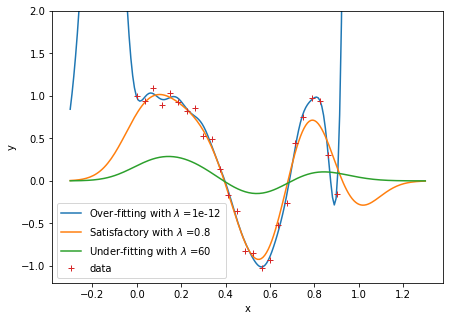
\includegraphics{../index3}	     
\end{center}

\subsection*{c)} Given :
\begin{equation*}
E = \frac{1}{D} \sum_{d=1}^{D} \frac{1}{N} \sum_{i=1}^{N} \left(y_i^d - y_i^{true} \right)^2
\end{equation*}
Where $y_i^{true} = \frac{1}{D} \sum_{d=1}^{D} y_i^d$
\subsubsection*{1)} Show that we can write E as :
\begin{equation*}
E = \frac{1}{D} \sum_{d=1}^{D} \frac{1}{N} \sum_{i=1}^{N} \left(y_i^d - y_i^{avg} \right)^2 + \frac{1}{N} \sum_{i=1}^{N} \left(y_i^{avg} - y_i^{true} \right)^2
\end{equation*}

we have :
\begin{align*}
E &= \frac{1}{D} \sum_{d=1}^{D} \frac{1}{N} \sum_{i=1}^{N} \left(y_i^d - y_i^{true} \right)^2 \\\\
  &= \frac{1}{D} \sum_{d=1}^{D} \frac{1}{N} \sum_{i=1}^{N} \left(y_i^d - y_i^{avg} +y_i^{avg} -  y_i^{true} \right)^2 \\\\
  &= \frac{1}{D} \sum_{d=1}^{D} \frac{1}{N} \sum_{i=1}^{N} \left(y_i^d - y_i^{avg}\right)^2 + \frac{1}{D} \sum_{d=1}^{D} \frac{1}{N} \sum_{i=1}^{N} \left(y_i^{avg} -  y_i^{true} \right)^2  + \underbrace{2\frac{1}{D} \sum_{d=1}^{D} \frac{1}{N} \sum_{i=1}^{N}  \left(y_i^{avg} -  y_i^{true} \right) \left(y_i^d - y_i^{avg}\right)}_{0}\\\\
  &= \frac{1}{D} \sum_{d=1}^{D} \frac{1}{N} \sum_{i=1}^{N} \left(y_i^d - y_i^{avg}\right)^2 +  \frac{1}{N} \sum_{i=1}^{N} \frac{1}{D} \sum_{d=1}^{D} \left(y_i^{avg} -  y_i^{true} \right)^2 \\
  &= \frac{1}{D} \sum_{d=1}^{D} \frac{1}{N} \sum_{i=1}^{N} \left(y_i^d - y_i^{avg}\right)^2 +  \frac{1}{N} \sum_{i=1}^{N} \frac{1}{D} D \left(y_i^{avg} -  y_i^{true} \right)^2 \\\\
  E &= \frac{1}{D} \sum_{d=1}^{D} \frac{1}{N} \sum_{i=1}^{N} \left(y_i^d - y_i^{avg}\right)^2 +  \frac{1}{N} \sum_{i=1}^{N} \left(y_i^{avg} -  y_i^{true} \right)^2
\end{align*}

So we have got : 
\begin{align*}
E &= \frac{1}{D} \sum_{d=1}^{D}\underbrace{ \frac{1}{N} \sum_{i=1}^{N} \left(y_i^d - y_i^{avg}\right)^2}_{bias} +  \underbrace{\frac{1}{N} \sum_{i=1}^{N} \left(y_i^{avg} -  y_i^{true} \right)^2}_{variance}
\end{align*}

From this equation , we can see that : \\ \\
The average squared error = variance + bias \\ \\

So :
\begin{itemize}
	\item When the Variance increase, the bias decrease because The average squared error is a positive value.
	\item When the Variance decrease, the bias increase.
\end{itemize}

This relation can be see as the bias-variance Trade-off

\section{Bayesian Linear Regression}
\subsection*{a)} Write a python function that lml(alpha, beta, Phi, Y) that returns the log marginal likelihood, and also a function grad ml(alpha, beta, Phi, Y) that returns the gradient of the marginal likelihood with respect to the vector $\alpha, \beta$. The function should return a numpy vector with the gradient with respect to $\alpha$ in the first component and gradient with respect to $\beta$ in the second. \\ \\

Our model is on the form : $y = \phi(x)w + \epsilon$ where $\epsilon \sim \mathcal{N}(0, \beta I)$ and the posterior is given by :
\begin{equation*}
p(w|y,x,\alpha, \beta) = \frac{p(y|w,\alpha,\beta,x)p(w)}{p(y|x)}
\end{equation*}

Where The marginal likelihood is given by:
\begin{equation*}
p(y|x,\alpha, \beta) = \int p(y, w|x, \alpha, \beta)dw = \int p(y| w,x,\alpha, \beta) p(w) dw
\end{equation*}

We have :
\begin{equation*}
p(y| w,x,\alpha, \beta) = \prod_{i=1}^{N} \mathcal{N}(y_i|w^T\phi_i)
\end{equation*}

\begin{equation*}
p(w) = \mathcal{N}(w|0,\alpha I)
\end{equation*}

So :
\begin{equation*}
p(y|x,\alpha, \beta) =\int \mathcal{N}(y|\phi w) \mathcal{N}(w|0,\alpha I) dw
\end{equation*}

This expression doesn't depend on $w$.\\

We will now compute it mean and covariance.\\
$E_w(y|X) = E_w(\phi(x)w + \epsilon) = \phi(x)E_w(w) = 0$\\ \\
$Cov_w(y) = Cov_w(\phi(x)w + \epsilon) = \phi (\alpha I) \phi^T + \beta I$ \\ \\
So the marginal likelihood is given by : 
\begin{equation*}
p(y|x,\alpha, \beta) = (2 \pi)^{-\frac{N}{2}} \arrowvert \alpha\phi\phi^T + \beta I \arrowvert^{-\frac{1}{2}} exp\left( -\frac{1}{2} y^T (\alpha\phi\phi^T + \beta I)^{-1} y\right)
\end{equation*}

The Log-Marginal likelihood is given by :
\begin{equation*}
log \, p(y|x,\alpha, \beta) = -\frac{N}{2} log 2\pi - \frac{1}{2}log\arrowvert \alpha\phi\phi^T + \beta I \arrowvert - \frac{1}{2} y^T (\alpha\phi\phi^T + \beta I)^{-1} y
\end{equation*}

Now , we will compute the gradient of the Log-Marginal likelihood with respect to $\alpha$ and $\beta$. \\\\
Let $A(\alpha,\beta) = \alpha\phi\phi^T + \beta I$, We can show that : 
\begin{equation*}
\frac{\partial}{\partial \alpha} det\, A(\alpha,\beta) = det\,A(\alpha,\beta) \,trace \left(A^{-1}(\alpha,\beta) \frac{\partial}{\partial \alpha}A(\alpha,\beta)\right)
\end{equation*}

\begin{equation*}
\frac{\partial}{\partial \alpha} A^{-1}(\alpha,\beta) = - A^{-1}(\alpha,\beta) \frac{\partial}{\partial \alpha} A(\alpha,\beta) A^{-1}(\alpha,\beta) 
\end{equation*}

So we can conclude that:
\begin{equation*}
\frac{\partial}{\partial \alpha} log \, p(y|x,\alpha, \beta) = -\frac{1}{2} \, trace \left[A^{-1}(\alpha,\beta) \phi \phi^T\right] + \frac{1}{2} y^T  A^{-1}(\alpha,\beta) \phi \phi^T A^{-1}(\alpha,\beta) y
\end{equation*}

\begin{equation*}
\frac{\partial}{\partial \beta} log \, p(y|x,\alpha, \beta) = -\frac{1}{2} \, trace \left[A^{-1}(\alpha,\beta)\right] + \frac{1}{2} y^T  A^{-1}(\alpha,\beta) A^{-1}(\alpha,\beta) y
\end{equation*}

\subsection*{b)} For the given data set and the linear basis functions (i.e. polynomial of order 1), maximize the log marginal likelihood with respect to $\alpha$ and $\beta$ using gradient descent. Show your steps on a contour plot. \\

For this experience, we found: \\
$\alpha_{max} = 0.4245549972256691$ and $\beta_{max} = 0.4492313296405098$ \\ \\ with the following parameters : 
\begin{itemize}
	\item learning rate = 0.01
	\item Size of the data set : N = 25
	\item The Data set : X = np.linspace(0,0.9,N).reshape(N,1)
	\item Y = f(X)
	\item We randomly initialize $\alpha$ and $\beta$
	\item We set-up the number of iteration : epoch = 1000
\end{itemize}

We obtain the following contour plot showing the convergence of to the maximum point $(\alpha_{max}, \beta_{max})$ : 

\begin{center}
	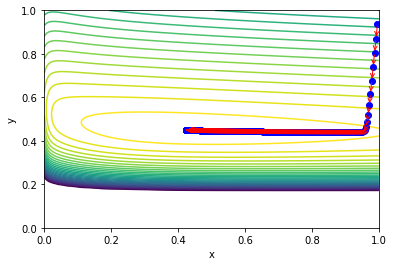
\includegraphics{../contour_plot.png}	     
\end{center}

\subsection*{c)} In the case of trigonometric basis function, compute the maximum of the log marginal likelihood for orders 0 to 11 inclusive using gradient descent (make sure you choose good starting values and a small step size with plenty of iterations). Plot these values on a graph against the order of the basis functions. Compare your answer to your cross validation graph from Question 1c) and describe briefly the merits of the two approaches.


\begin{center}
	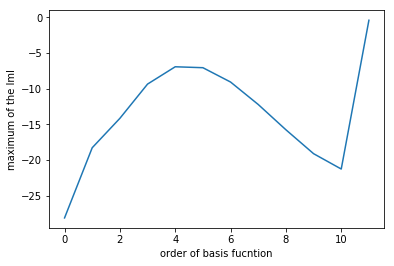
\includegraphics{../3c.png}	     
\end{center}

From Question 1c) we can see that a good choose of the degree of the polynomial is 4 and in fact it 'is confirmed in this graph we can see that the maximum value of the log marginal likelihood for orders 0 to 11 is reach for the degree of the polynomial equal to 4, But this method is more accurate because we are using here the gradient descent method, hence we are sure about the convergence or the maximum of the log marginal likelihood.

\subsection*{d)}
\begin{center}
	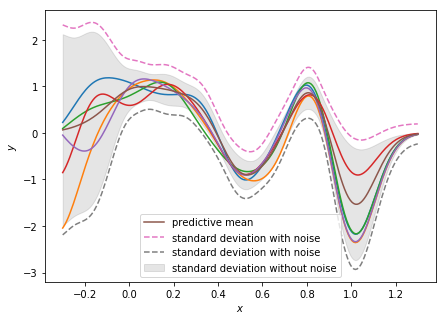
\includegraphics{../3d.png}	     
\end{center}
\end{document}
